\section{Theoretische Grundlage}
\label{sec:Theorie}

\subsection{Einführung}
Ist in einem Raum keine Matereie vorhanden und der Gasdruck verschwunden, wird dieser als perfektes Vakuum betitelt. Bereits die griechischen Philiosophen ende des 4 Jahrhundert konnten die Gedankenspiele über die Existenz eines eines leeren Raums nicht zweifelsfrei beantworten. Mit dem Aufstreben der Quantenmechanik, stellt sich erneut die Frage in wie fern überhaupt ein Teilchenfreier Raum in grenzen der Energie-Zeitunschärfe möglich ist, worauf im folgenden noch eingenangen wird. Rein phänomenologisch ist das Vakuum definiert als:

``\textit{Vakuum heißt der Zustand eines Gases, wenn in einem Behälter der Druck des Gases und damit die Teilchenzahldichte niedriger ist als außerhalb oder wenn der Druck des Gases niedriger ist als 300 mbar, d. h. kleiner als der niedrigste auf der Erdoberfläche vorkommende Atmosphärendruck}'' \cite{DIN}

Ziel des Versuches ist es die Grundlagen der Vakuumstechnik nachzuvollziehen und die für den Versuch benötigten Komponenten kennenzulernen. Dies geschieht indem für die beiden verwendeten Pumpenarten die Saugleistung, als auch eine Leckratenmessung durchgeführt wird.

\subsection{Mesgrößen zur Bestimmung des Vakuums}
Das Maß eines Vakuums ist der Druck $p$. Dieser ist definiert als Kraft $F$ pro Fläche $A$
\begin{equation}
  p = \frac{F}{A} = \left[ \frac{N}{m^2} \right]
  \label{eqn:druck}
\end{equation}
Anhand dessen lassen sich Vakuums in verschiedene Kategorien unterteilen, was im späteren noch passieren wird. Desweiteren lässt sich bei einem gemsich aus Gasen der Gesamtdruck $p_\text{Ges}$ in mehre Partialdrücke aufteilen. Es gilt immer, dass die Summe über alle partialdrücke dem Gesamtdruck entspricht. Analog wird mit der Teilchenanzahl vorgegangen. Der Partialdruck entspricht dem Druck welcher das entsprechende gemisch in dem selben Volume wodrin sich $p_\text{Ges}$ befindet ausübern würde. \newline
Einheiten \newline
Desweiteren zeichnet sich ein Gas durch die mittlere freie Weglänge $\Lambda$ eines Teilcens aus, bis es mit einem anderen wechselwirkt. Durch einführen eines Stoßquerschnitts und einer konstanten Teilchenzahldichte $n$ lässt sich durch lösen einer Differentialgleichung 
\begin{equation}
  \frac{dN}{N} = -n \sigma \Delta x
  \label{eqn:mfWDGL}
\end{equation}
zeigen, dass die mittlere freie Weglänge  inversproportional zu dem Produkt aus Teilchenzahlichte und Stoßquerschnitt ist.
\begin{equation}
  \Lambda = \frac{1}{n \sigma}= \frac{k T}{\sqrt{2} \pi D^2 p}
  \label{eqn:mfW}
\end{equation}
Da die Teilchenanzahl von Luft bei Normaldruck als gegeben vorrausgesetzt wird kann aus der Vorraussetzung, dass das Produkt aus pV =const ist die Teilchenzahl bei den anderen Drücken berechnet werden. 
\begin{table}
  \centering
  \caption{Druckbereiche, Mittlere Freie Weglänge und Teilchenanzahl}
  \begin{tabular}{c|c c c}
  	\toprule
	Druckbereiche & Druck / mbar & Moleküle / $cm^3$ & mittlere freie Weglänge \\
	\midrule
	Normaldruck	& 1013.25			& $2.7 \cdot 10^{19}$ &	68 nm \\
	Unterdruck	& > 300				& k.A. & k.A \\
	Grobvakuum	& 300 \ldots 1 			&$10^{19} \cdot 10^{16}$&0.1 \ldots 100 $\mu m$ \\
	Feinvakuum	& 1 \ldots $10^{-3}$		& $10^{16} \cdot 10^{13}$ & 0.1 \ldots 100 mm \\
	Hochvakuum	& $10^{-3} \cdots 10^{-7}$	& $10^{13} \cdot 10^{9}$ & 100 mm \ldots 1km \\
	Ultrahochvakuum	& $10^{-7} \cdots 10^{-12}$	& $10^9 \cdots 10^4$ & 1 m \ldots $10^5$ m \\
	extrem hohes Vakuum & $< 10^{-12}$		& $<10^4$ & $> 10^5$ \\
	\bottomrule
  \end{tabular}
  \label{tab:ueberblick}
\end{table}


Ausgasen


\subsection{p(t) Kurve}
Für die Auswertung wird eine Funktion benötigt welche den Druck in abhängigkeit der Zeit angibt. Dafür muss die Annahme getroffen werden, dass die Saugleistug $S$ für den anegebenen Zeitraum konstant ist und nicht vom Druck $p(t)$ abhängt. Dann entspricht die zeitliche Änderung des Volumens 
\begin{equation}
  \frac{\text{d}V}{\text{d}t} = S \ .
\end{equation}
Zusätzlich wird eingefordert das die Temperatur des Gases bei dem Vorgang konstant ist. Mithilfe des idealen Gasgesetz
\begin{equation}
  p V = n R T
\end{equation}

\begin{equation}
  \frac{\text{d}}{\text{dt}} pV = \frac{\text{d}}{\text{dt}} n R T
\end{equation}

\begin{equation}
  p(t) = p_0 \exp \left( \frac{-t}{\tau} \right)
\end{equation}
Durch einsetzen der Anfangsbedingungen und des Enddrucks $p_\text{E}$ ergibt sich für den Zeitabhängigen Druck 
\begin{equation}
  p(t) = (p_0 - p_\text{E}) \exp \left( -t \frac{S}{V} \right) + p_\text{E}
\end{equation}

\subsection{Wechselwirkungsprozesse Restgas Umgebung}
Befindet sich ein Gas oder eine Flüssigkeit eingeschloßen in einem Körper, wechseltwirkt diese mit der Grenzfläche. Dabei können die aufgeführten Prozesse auftreten und die Messreihe beeinflussen. In Kapitel \ref{??} werden Maßnahmen vorgestellt dem entgegenzuwirken. (Phönen, Rezipient verschließen).
\begin{itemize}
  \item \textbf{Absorption:} Trifft ein Teilchen auf die Grenzfläche, kann es passieren das es von dieser aufgenommen wird. Dannach befindet es sich für unestimmte Zeit im Absorbermaterial, kan jedoch auch wieder Reduktieren.
  \item \textbf{Adsorption:} Trifft ein Teilchen auf die Grenzfläche kann es neben der Absorbtion sich auch am Rand des Absorbermaterials ablagern. Dabei wird es mittels der Van-der-Waals kräfte am Rand lokalisiert.
  \item \textbf{Desorption:} Es ist der Umkehrprozess der Absorbtion. Dabei wird ein Teilchen aus des Rezipienten an das Vakuum abgegeben und ist somit nicht mer lokalisiert. 
  \item \textbf{Diffusion:} Ist in einem geschlossenen System eine inhomogenen Gasverteilung, sorgt die Diffusion dafür das die Verteilung in den Gleicgewichtszustand über geht. Es beruht darauf das die ungerichteten Bewegungen die Zeitunkehrinvarianz brechen und das System in den Zustand der maximalen Entropie treibt.
  \item \textbf{Ausgasen:} Ist ein Festkörper durch zu langen kontakt mit der Umwelt verureinigt, muss bei diesem die Gasteilchen zunächst ersteinmal an die Oberfläche diffundieren bevor sie desobiert werden können. dadurch kann nicht so schnell der Sättigungswert für die Pumpen errreicht werden.
\end{itemize}
\subsection{Ströungsprozesse und Leitwert}

Laminare Strömung:

molekulare Strömung:

Leitwert:


\section{Technische Grundlagen}

\subsection{Pumpentypen und Funktionsweise}

Drehschieberpumpe:
\begin{figure}[H]
    \centering
    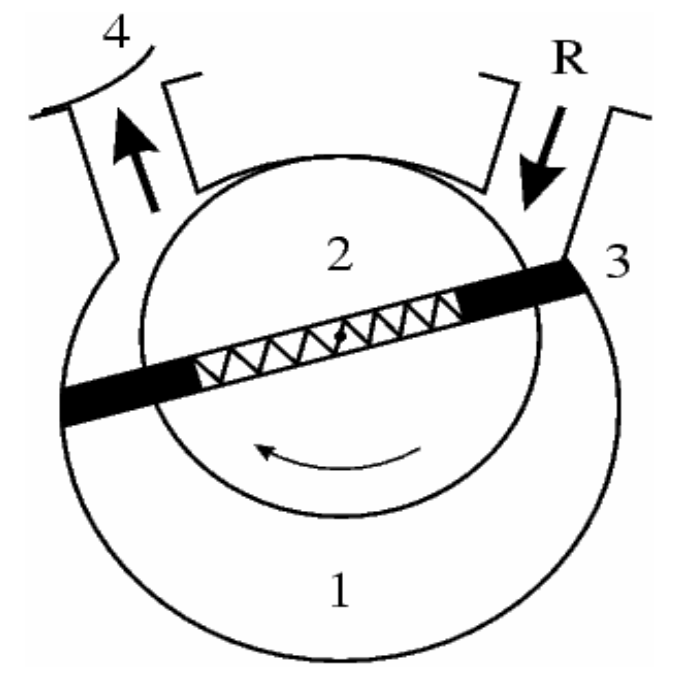
\includegraphics[width=0.3\textwidth]{./picture/Drehschieberpumpe.png}
    \caption{<+caption text+>}
    \label{fig:<+label+>}
\end{figure}

Turbopumpe:
\begin{figure}[H]
    \centering
    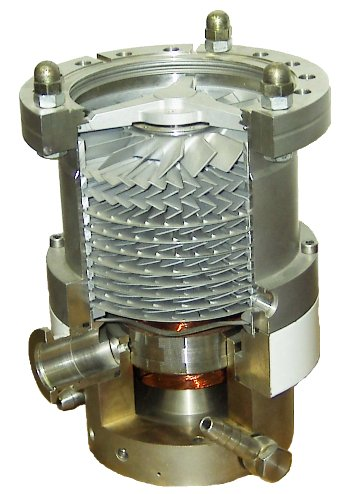
\includegraphics[width=0.3\textwidth]{./picture/Turbo.jpg}
    \caption{<+caption text+>}
    \label{fig:<+label+>}
\end{figure}


\subsection{Messgeräte}

Pirani-Messgerät


Kaltkatohden-Messgerät

Heißkathonden-Messgerät

\section{Fehlerrechnung}
Sämtliche Fehlerrechnungen werden mit Hilfe von Python 3.4.3 durchgeführt.
\subsubsection{Mittelwert}
Der Mittelwert einer Messreihe $x_\text{1}, ... ,x_\text{n}$ lässt sich durch die Formel
\begin{equation}
	\overline{x} = \frac{1}{N} \sum_{\text{k}=1}^\text{N} x_k
	\label{eqn:ave}
\end{equation}
berechnen. Die Standardabweichung des Mittelwertes beträgt
\begin{equation}
	\Delta \overline{x} = \sqrt{ \frac{1}{N(N-1)} \sum_{\text{k}=1}^\text{N} (x_\text{k} - \overline{x})^2}
	\label{eqn:std}
\end{equation}

\subsubsection{Gauß'sche Fehlerfortpflanzung}
Wenn $x_\text{1}, ..., x_\text{n}$ fehlerbehaftete Messgrößen im weiteren Verlauf benutzt werden, wird der neue Fehler $\Delta f$ mit Hilfe der Gaußschen Fehlerfortpflanzung angegeben.
\begin{equation}
	\Delta f = \sqrt{\sum_{\text{k}=1}^\text{N} \left( \frac{ \partial f}{\partial x_\text{k}} \right) ^2 \cdot (\Delta x_\text{k})^2}
	\label{eqn:var}
\end{equation}

\subsubsection{Lineare Regression}
Die Steigung und y-Achsenabschnitt einer Ausgleichsgeraden werden gegebenfalls mittels Linearen Regression berechnet.
\begin{equation}
	y = m \cdot x + b
	\label{eqn:reg}
\end{equation}
\begin{equation}
	m = \frac{ \overline{xy} - \overline{x} \overline{y} } {\overline{x^2} - \overline{x}^2}
	\label{eqn:reg_m}
\end{equation}
\begin{equation}
	b = \frac{ \overline{x^2}\overline{y} - \overline{x} \, \overline{xy}} { \overline{x^2} - \overline{x}^2}
	\label{eqn:reg_b}
\end{equation}
